\documentclass[tikz,border=6pt]{standalone}
\usetikzlibrary{arrows.meta}

\definecolor{conceptred}{HTML}{C83E3A}
\definecolor{axisgray}{HTML}{3F4650}
\definecolor{pointgray}{HTML}{B8BEC7}
\definecolor{roundblue}{HTML}{3973A8}

\tikzset{
  point/.style={draw=axisgray, line width=.35pt, minimum size=4.2pt, inner sep=0pt},
  neither/.style={point, rectangle, fill=pointgray},
  redonly/.style={point, rectangle, fill=conceptred},
  roundonly/.style={point, circle, fill=pointgray},
  redround/.style={point, circle, fill=conceptred},
  estimate/.style={-{Latex[length=2.4mm]}, line width=1.25pt}
}

\begin{document}
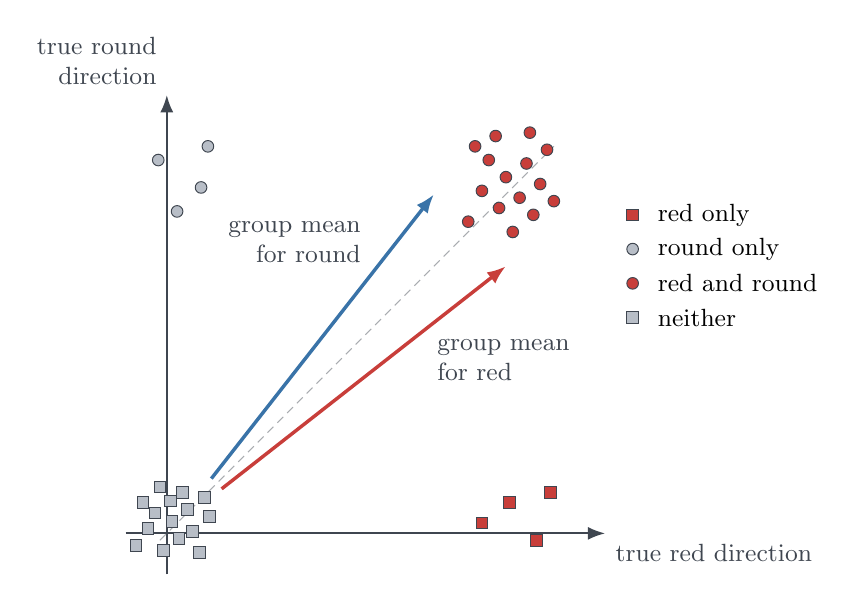
\begin{tikzpicture}[x=4.35cm,y=4.35cm,font=\small]
  % The true representation has two orthogonal concept axes.
  \draw[-{Latex[length=2.2mm]},line width=.8pt,axisgray]
    (-.12,0) -- (1.28,0) node[below right] {true red direction};
  \draw[-{Latex[length=2.2mm]},line width=.8pt,axisgray]
    (0,-.12) -- (0,1.28) node[above left,align=right] {true round\\direction};
  \draw[densely dashed,axisgray!45] (-.02,-.02) -- (1.13,1.13);

  % Many neither and red+round samples, but few red-only or round-only samples.
  \foreach \x/\y in {
    -.055/.015,-.035/.060,-.010/-.050,.015/.035,.035/-.015,
    .060/.070,.075/.005,.010/.095,-.070/.090,.095/-.055,
    -.090/-.035,.045/.120,-.020/.135,.125/.050,.110/.105}
    \node[neither] at (\x,\y) {};

  \foreach \x/\y in {.92/.03,1.00/.09,1.08/-.02,1.12/.12}
    \node[redonly] at (\x,\y) {};

  \foreach \x/\y in {.03/.94,.10/1.01,-.025/1.09,.12/1.13}
    \node[roundonly] at (\x,\y) {};

  \foreach \x/\y in {
    .88/.91,.92/1.00,.94/1.09,.97/.95,.99/1.04,
    1.01/.88,1.03/.98,1.05/1.08,1.07/.93,1.09/1.02,
    1.11/1.12,1.13/.97,.90/1.13,.96/1.16,1.06/1.17}
    \node[redround] at (\x,\y) {};

  % Marginal group-mean differences are rotated toward the diagonal.
  \draw[estimate,conceptred]
    (.16,.13) -- (.99,.78)
    node[pos=.72,below right,align=left,text=axisgray] {group mean\\for red};
  \draw[estimate,roundblue]
    (.13,.16) -- (.78,.99)
    node[pos=.72,above left,align=right,text=axisgray] {group mean\\for round};

  % Compact visual legend: red fill means red; circular shape means round.
  \begin{scope}[shift={(1.36,.93)}]
    \node[redonly] at (0,0) {};
    \node[anchor=west] at (.045,0) {red only};
    \node[roundonly] at (0,-.10) {};
    \node[anchor=west] at (.045,-.10) {round only};
    \node[redround] at (0,-.20) {};
    \node[anchor=west] at (.045,-.20) {red and round};
    \node[neither] at (0,-.30) {};
    \node[anchor=west] at (.045,-.30) {neither};
  \end{scope}
\end{tikzpicture}
\end{document}
